%*******************************************************************************
%*********************************** Third Chapter *****************************
%*******************************************************************************

\chapter{Fine-grained Recognition}
\label{chap:finegrained_classification}

%% Write about Paper A and B in a coherent way

This chapter presents an approach for enhancing fine-grained classification performance of grocery items by using web-scraped information. We focus on classification of grocery items due to applicability in assistive vision and its potential to enhance the independence of visually impaired (VI) people [ADD groceries/shopping/object recognition for VI REFs]. Initially, we were interested in learning classifiers with natural images taken in the grocery stores combined with web-scraped information about the grocery items, such as iconic images and text descriptions from supermarket websites. Using iconic images have been used in grocery image classification earlier [ADD grocery paper REFs], however, utilizing text descriptions was as far we know absent for this application even if it has been successfully applied in other image classification problems~\cite{wah2011cub, nilsback2008automated, bujwid2021large}. Thus, we collected our own dataset of grocery items images using a mobile phone camera as well as web-scraped images and text descriptions to study whether this multi-view approaches would benefit training the classifiers (Section 2). We then select a multi-view learning framework based on the Variational Autoencoder (VAE) for investigating how the different data views affect the fine-grained classification performance (Section 3). 

%\section{Introduction}
\section{Related Work}

In this section, we will briefly discuss the related work on fine-grained image recognition~\cite{wei2021fine}, particularly when learning from external information, and multi-view learning. 

\subsection{Fine-grained Image Recognition}
%\paragraph{Fine-grained Image Recognition.} 
The goal with fine-grained image recognition (FGIR) is to distinguish between images with multiple visually similar sub-categories that belong to a super-category. For example, various attempts have been made to discriminate between sub-categories of different animals~\cite{van2018inaturalist}, cars~\cite{krause2013stanford_cars}, fruits~\cite{hou2017vegfru}, retail products~\cite{wei2019rpc}, etc. The challenge is to recognize differences that are sufficient for discriminating between objects that are generally similar but differ in fine-grained visual details. In recent years, the successes with deep learning in computer vision have encouraged researchers to explore various approaches for FGIR that can broadly be divided into three directions for recognition by utilizing (i) localization-classification subnetworks, (ii) end-to-end feature encoding, and (iii) external information. In (i), the goal is to find object parts that are shared across the sub-categories for discovering details that make the part representations different. This can be achieved by utilizing feature maps from the activations of convolutional layers as local descriptors~\cite{zhang2016picking, wang2018learning, ding2019selective}, employing detection and segmentation techniques for localizing object parts[REFs], or leveraging attention mechanisms when common object parts are difficult to represent or even define [REFs]. With (ii), the goal has been to learn features that are better at capturing subtle and local differences by, for instance, performing high-order features interactions~\cite{lin2015bilinear} as well as designing novel loss functions [Add REFs]. In the third approach (iii), the goal is to leverage external information, for example, web data and multimodal data, in FGIR as additional supervision to the images. We will put more focus on the approach on FGIR with external information next, as we use this approach in Paper A and B. 

\subsection{Recognition with External Information}
%\paragraph{Recognition with External Information.} 
Learning fine-grained details about objects often requires large amounts of labeled data. To ease the need for large amounts of accurately labeled images, there have been several attempts to let either web-scraped or multimodal data influence learning the fine-grained features of the sub-categories to boost the FGIR performance. Web-scraped images may be noisy in the sense that retrieved images may have high-variations of the objects. For example, the objects of interest can look different in appearance, and there could also be other irrelevant objects in the images that potentially occlude the category to recognize. Hence, incorporating web-scraped data into the training set may establish a domain gap between the easily acquired web data and the original training set which we need to overcome by reducing the domain gap or reducing the negative effects of the noisy web data that can disturb the learning. Another direction than using web-scraped data is to utilize multimodal data, for example, images, text and knowledge bases, for boosting the classification performance. In FGIR, the goal is to establish a joint representation between the images and additional data sources, where the additional data should act like extra guidance for learning useful representations that capture the fine-grained details of objects. Text descriptions have been a popular data type to combine with images, which can be both easy and cheap to collect as they can be accurately generated by non-experts. High-level knowledge graphs of objects have also been used and can contain rich knowledge useful for fine-grained recognition. In addition to FGIR, both web-scraped and multimodal external information has been used for zero-shot learning to transfer knowledge from annotated categories to new fine-grained categories. In Paper A, we collect web-scraped images and text descriptions of grocery items to accompany real-world images of groceries for FGIR. Then, in Paper B, we perform a study using multi-view learning to investigate how the external information can enhance the classification performance. Next, we will cover the related work for the multi-view learning approach that we used. 


\subsection{Multi-view Learning}
%\paragraph{Multi-view Learning.} 
Learning from several data sources and modalities % CCA, Autoencoders, VCCA, multimodal VAEs



%There exist lots of multi-view learning approaches for data fusion of multiple features~\cite{baltruvsaitis2018multimodal, cremer2018importance, frome2013DeVISE, fu2016semi, karpathy2015deep, ngiam2011multimodal, pieropan2014audio,  salzmann2010factorized, shi2019variational, suzuki2016joint, tsai2018learning, vedantam2017generative, wang2016deep, wu2018multimodal, xian2018zero, xu2013survey, zhang2016inter, zhao2017multi}. A common approach is to obtain a shared latent space for all views with the assumption that each view has been generated from this shared space~\cite{xu2013survey}. A popular example of this is approach is Canonical Correlation Analysis (CCA)~\cite{hotelling1936relations}, which aims to project two sets of variables (views) into a lower-dimensional space so that the correlation between the projections is maximized. Similar methods propose maximizing other alignment objectives for embedding the views, such as ranking losses~\cite{frome2013DeVISE, fu2016semi, karpathy2015deep, xian2018zero}. 
%There exist nonlinear extensions of CCA, e.g., Kernel CCA~\cite{akaho2006kernel} and Deep CCA~\cite{andrew2013deep}, that optimize their nonlinear feature mappings based on the CCA objective. 
%Deep Canonically Correlated Autoencoders (DCCAE)~\cite{wang2015deep} is a Deep CCA model with an autoencoding part, which aims to maximize the canonical correlation between the extracted features as well as reconstructing the input data. 
%Removing the CCA objective reduces DCCAE to a standard multi-view autoencoder, e.g., Bimodal Autoencoders and Split Autoencoders (SplitAEs)~\cite{ngiam2011multimodal, wang2015deep}, that only aim to learn a representation that best reconstructs the input data. SplitAEs aim to reconstruct two views from a representation encoded from one of the views. This approach was empirically shown to work better than Bimodal Autoencoders in \cite{ngiam2011multimodal} in situations where only a single view is present at both training and test time.

%Variational CCA (VCCA)~\cite{wang2016deep} can be seen as an extension of CCA to deep generative models, but can also be described as a probabilistic version of SplitAEs.
%VCCA uses the amortized inference procedure from Variational Autoencoders (VAEs)~\cite{kingma2013auto, zhang2018advances} to learn the shared latent space by maximizing a lower bound on the data log-likelihood of the views. Succeeding works have proposed new learning objectives and inference methods for enabling conditional generation of views, e.g., generating an image conditioned on some text and vice versa~\cite{cremer2018importance, shi2019variational, suzuki2016joint, vedantam2017generative, wu2018multimodal}. These approaches rely on fusing the views into the shared latent space as the inference procedure, which often requires tailored training and testing paradigms when views are missing. However, adding information from multiple views may not lead to improved results and can even make the model perform worse on the targeted task~\cite{guler2014whats, ngiam2011multimodal}. This is especially the case when views have noisy observations, which complicates learning a shared latent space that combines the commonalities between the views. To avoid disturbing the shared latent space with noise from single views, some works design models which extend the shared latent space with private latent spaces for each view that should contain the view-specific variations to make learning the shared variations easier~\cite{hyvarinen2000independent, salzmann2010factorized, tsai2018learning, wang2016deep, zhang2016inter}. VCCA can be extended to extract shared and private information between different views through factorization of the latent space into shared and private parts. In this paper, we investigate if the classification performance of grocery items in natural images can be improved by extracting the view-specific variations in the additional views (iconic images and product descriptions) from the shared latent space with this variant of VCCA called VCCA-private. We will experiment with treating each data point as pairs of natural images and either iconic images or text descriptions as well as triplets of natural images, iconic images, and text descriptions.
%A difference between how we apply VCCA to our dataset compared to the works above is that the iconic image and text description are the same for every natural image of a specific class.  



%Adding web-scraped data of the categories of interest to the training data is referred to as \textit{webly supervised learning}  

%There have been several attempts to utilize external information, for example, web images, to enhance the performance of FGIR. % How are we different from other works that used web information for recogntion? This can be on dataset level. But also describe some approaches and then that we use multi-view learning. 


\section{Dataset Collection}
In this section, we describe our procedure for collecting the image dataset of grocery items. As the target use case is grocery shopping with an assistive vision device, we visited several supermarkets and collected natural images of the groceries with a mobile phone camera to imitate such scenarios. Hence, the collected images will capture situations that can be challenging for the assistive device, such as, various lighting conditions, multiple instances and classes present, hand occlusions, and misplaced items. All images were taken with a single targeted item in mind, such that each image is paired with a single label. For items which belong to a clear super-class, for example, various kinds of apples and milk packages, we also provided the general class of the items to establish a hierarchical labeling structure of the data. Collecting natural images of the grocery items is unfortunately a time-consuming process. Furthermore, as the surroundings in every grocery store varies, it may be difficult to build accurate classifiers that can recognize fine-grained details solely from natural images. Hence, we need some cheaper procedure that can complement the collection of real-world images for boosting the classification performance of the groceries. 

We have complemented the image dataset with external information from the web of each grocery item that can be used for training classifiers. In the past years, most supermarket chains have the option for consumers to purchase groceries online from their websites. The website usually provides each grocery item with an iconic image of the item on a white background, a text description that describes the flavor and ingredients of the item, as well as nutrition values if applicable. We downloaded these information types of all grocery item classes by web-scraping the online shopping website of a supermarket chain. We show four examples of grocery items and their web-scraped information in Table \ref{tab:grocery_store_dataset}. Since these data types are on a class-based level, we can use the web-scraped information as weak supervision to guide the classifier to learn fine-grained details that helps discriminating between visually similar items.   

\begin{table}[t]
	\centering
	\caption{\small{ Examples of grocery item classes in the Grocery Store dataset. We display four different items (coarse-grained class in parenthesis), followed by two natural images taken with a mobile phone inside grocery stores. Next comes the web-scraped information of the items consisting of an iconic image and a text description. We have highlighted ingredients and flavors in the text description that are characteristic for the specific item. }}
	\vspace{-10pt}
	\setlength{\fboxsep}{0pt} 
	\setlength{\fboxrule}{0.33pt}
	

	%\resizebox{0.98\textwidth}{!}{
	\begin{tabular}{c | c | c | c}
	\hline
	\thead{\footnotesize Class \\ \footnotesize Labels} & \thead{\footnotesize Natural \\ \footnotesize Images} & \thead{\footnotesize Iconic \\ \footnotesize Images} & \thead{\footnotesize Text \\ \footnotesize Descriptions} \\
	\hline 
	\makecell{ \scriptsize Granny Smith \\[-1pt] \scriptsize (Apple)}
	&  \makecell{ \begin{tikzpicture}
			\begin{scope}
				\node {\fbox{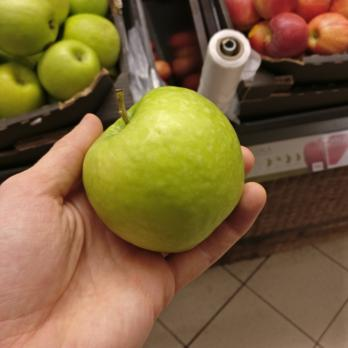
\includegraphics[width=30pt]{Chapter1/pics/Granny-Smith_021.jpg}}};
			\end{scope}
			\begin{scope}[xshift=34pt]
				\node {\fbox{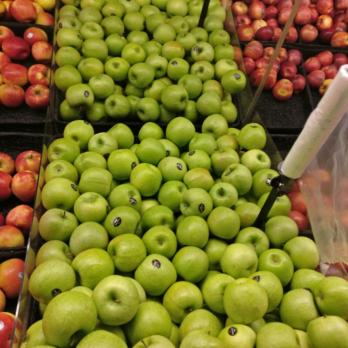
\includegraphics[width=30pt]{Chapter1/pics/Granny-Smith_012.jpg}}};
			\end{scope}
	\end{tikzpicture} }& 
	\makecell{\begin{tikzpicture}
			\begin{scope}
				\node {\fbox{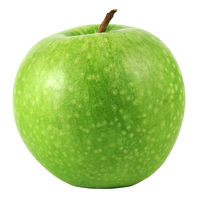
\includegraphics[width=30pt]{Chapter1/pics/Granny-Smith_Iconic.jpg}}};
			\end{scope}
	\end{tikzpicture} } & 
	\begin{scriptsize}
		\makecell{ \textit{“…green apple with white, firm pulp } \\[-1pt]  \textit{and a clear acidity in the flavor.”} } 
	\end{scriptsize}
	\\
	\hline 
	\makecell{ \scriptsize Royal Gala \\[-1pt] \scriptsize (Apple)}
	&  \makecell{ \begin{tikzpicture}
			\begin{scope}
				\node {\fbox{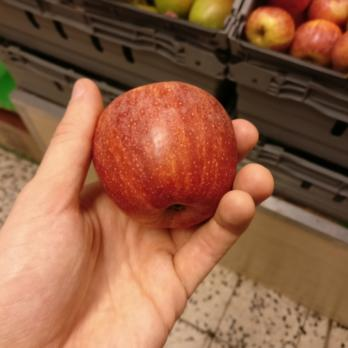
\includegraphics[width=30pt]{Chapter1/pics/Royal-Gala_005.jpg}}};
			\end{scope}
			\begin{scope}[xshift=34pt]
				\node {\fbox{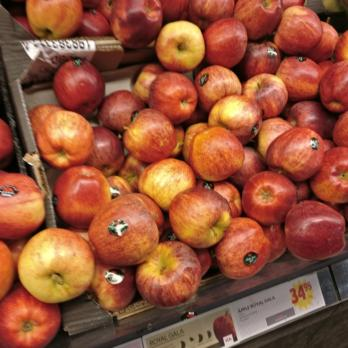
\includegraphics[width=30pt]{Chapter1/pics/Royal-Gala_002.jpg}}};
			\end{scope}
	\end{tikzpicture} }& 
	\makecell{\begin{tikzpicture}
			\begin{scope}
				\node {\fbox{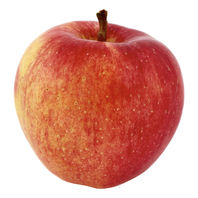
\includegraphics[width=30pt]{Chapter1/pics/Royal-Gala_Iconic.jpg}}};
			\end{scope}
	\end{tikzpicture} } & 
	\begin{scriptsize}
		\makecell{ \textit{“…crispy and very juicy apple,} \\[-1pt] \textit{with yellow-white pulp. The peel} \\[-1pt] \textit{is thin with a red yellow speckled color.”} } 
	\end{scriptsize}
	\\
	\hline
	\makecell{ \scriptsize Tropicana \\[-1pt] \scriptsize Mandarin \\[-1pt] \scriptsize (Juice)}
	&  \makecell{ \begin{tikzpicture}
			\begin{scope}
				\node {\fbox{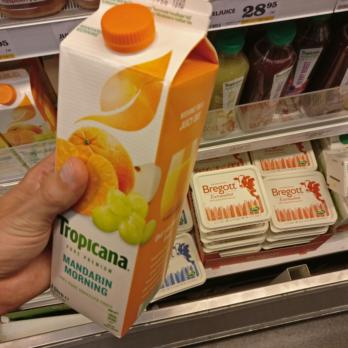
\includegraphics[width=30pt]{Chapter1/pics/Tropicana-Mandarin-Morning_003.jpg}}};
			\end{scope}
			\begin{scope}[xshift=34pt]
				\node {\fbox{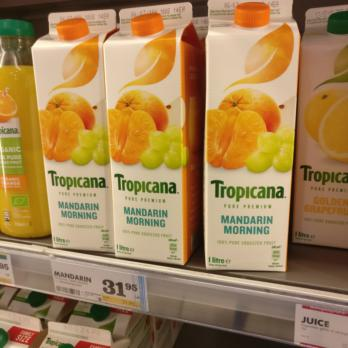
\includegraphics[width=30pt]{Chapter1/pics/Tropicana-Mandarin-Morning_016.jpg}}};
			\end{scope}
	\end{tikzpicture} }& 
	\makecell{\begin{tikzpicture}
			\begin{scope}
				\node {\fbox{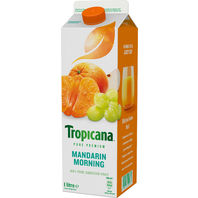
\includegraphics[width=30pt]{Chapter1/pics/Tropicana-Mandarin-Morning_Iconic.jpg}}};
			\end{scope}
	\end{tikzpicture} } & 
	\begin{scriptsize}
		\makecell{ \textit{“…is a ready to drink juice} \\[-1pt]
			\textit{without pulp pressed on orange,} \\[-1pt]
			\textit{ mandarin and grapes. Not from} \\[-1pt]
			\textit{concentrate. Mildly pasteurized.” } }
	\end{scriptsize}
	\\
	\hline
	\makecell{ \scriptsize Yoggi Vanilla \\[-1pt] \scriptsize (Yoghurt)}
	&  \makecell{ \begin{tikzpicture}
			\begin{scope}
				\node {\fbox{
\includegraphics[width=30pt]{Chapter1/pics/Yoggi-Vanilla-Yoghurt_001.jpg}}};
			\end{scope}
			\begin{scope}[xshift=34pt]
				\node {\fbox{
\includegraphics[width=30pt]{Chapter1/pics/Yoggi-Vanilla-Yoghurt_010.jpg}}};
			\end{scope}
	\end{tikzpicture} }& 
	\makecell{\begin{tikzpicture}
			\begin{scope}
				\node {\fbox{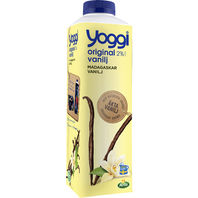
\includegraphics[width=30pt]{Chapter1/pics/Yoggi-Vanilla-Yoghurt_Iconic.jpg}}};
			\end{scope}
	\end{tikzpicture} } & 
	\begin{scriptsize}
		\makecell{ \textit{“...creamy vanilla yoghurt} \\[-1pt]
			\textit{original... added sugar than  } \\[-1pt]
			\textit{regular flavored yoghurt. Great for } \\[-1pt]
			\textit{both breakfast and snacks.”}}
	\end{scriptsize}
	\\
	\hline
\end{tabular}
%}
	\label{tab:grocery_store_dataset}
	%\vspace{-7mm}
\end{table}


\section{Multi-view Representation Learning of Grocery Items}

This section describes the approach we took for learning representations of grocery items that are shared across the available data types. We employ a deep latent variable model called Variational Canonical Correlation Analysis~\cite{wang2016deep} (VCCA) for learning the shared representation. The main assumption in VCCA is that each data view have been generated from the same latent space. The goal then is to learn this latent space that captures the correspondences between all views into representations shared across the views for the grocery items. This representation can then be utilized for enhance the learning more accurate classifiers as well as for performing tasks such as synthesis and prediction of novel images. Next, we describe how to enable learning the shared latent space. 

Capturing variations from each view in the learned representation is performed by predicting the original views from the latent space. To obtain the latent representation, we extract the representation by encoding the natural images with neural network. The extracted representation is then used for predicting each view individually by inputting the representation through separate neural networks. Note that we only use the natural images for extracting the latent representation here since it is the only view that is available at test time when we want to use the learned classifier in the grocery store. We have two options for exploiting the new representation to train classifiers. The first option is to train the classifier with the latent representations after we have learned the latent space as described above. The second option is to train the classifier and learning the latent space simultaneously by adding an additional classifier network predicting the class label with the latent representation as input. 

\MK{TO-DO: Need to introduce the ELBO. I should also add a figure of the architecture for extra clarity on the method. }
%Latent variable models similar to VCCA have been successful in applications where some views are on class-specific levels and the same across all instances of the class. An example of such view could be the label of a digit or letter, as well as the attributes of animals that are the same for all images of every class in the datasets~\cite{wah2011cub, lampert2009learning}. 

% where we can exploit the new representation to learn more accurate classifiers. 

%The new representation can be used for learning more accurate classifiers.  

 

%The architecture that we used is shown in Figure X.   

%learning joint representation of the different data types.

%we take an encoder-decoder approach as these have been successful in applications with data with images and class-specific additional data types. this is in contrast to webly supervised methods where the web data usually has many instances per class. 

%we use shared subspace learning approach from multi-view learning because it is a simple approach that gives us a joint representation across the views that we can use for training classifiers. This also opens up for using generative modeling approaches 


\section{Experiments}
\section{Discussion}


\noindent 
%In this chapter, we provide a summaries of the included paper for this thesis. Paper \ref{sec:paperA} and \ref{sec:paperB} are connected through the Grocery Store dataset where we present the work and then perform an ablation study over which modalities in the dataset that are useful for training classifiers. In Paper \ref{sec:paperC} and \ref{sec:paperD}, we focus on continual learning (CL) and present a new setting that aims to fill the gap between CL research and real-world problems as well as a method for doing so. 

%\begingroup
%\renewcommand\thesection{\Alph{section}} % for changing section numbering to alphabetic
%
\section{A Hierarchical Grocery Store Image Dataset with Visual and Semantic Labels}
\label{sec:paperA}

\textbf{Authors:} Marcus Klasson, Cheng Zhang, Hedvig Kjellström. 

\paragraph{Summary.} 
We collect a dataset with natural images of raw and refrigerated grocery items taken in grocery stores in Stockholm, Sweden, for evaluating image classification models on a challenging real-world scenario. The data collection was performed by taking photos of groceries with a mobile phone to simulate a scenario of grocery shopping using an assistive vision app. Furthermore, we downloaded iconic images and text descriptions of each grocery item by web-scraping a grocery store website to enhance the dataset with information describing the semantics of each individual item. the items are grouped based on their type, e.g., apple, juice, etc., to provide the dataset with a hierarchical labeling structure. 

We provide benchmark results evaluated using pre-trained and fine-tuned CNNs for image classification. Moreover, we take an initial step towards utilizing the rich product information in the dataset by training the classifiers with representations where both natural and iconic images have been combined through a multi-view VAE. 



\paragraph{Author Contributions.} CZ and HK presented the idea and the data collection procedure for the natural images and web-scraped information. MK performed the data collection including visiting the grocery stores for taking the natural images and the web-scraping of the grocery store website for iconic images and text descriptions. MK performed all the experiments. All authors contributed to discussing the results and contributed to writing the manuscript. 


%
\section{Using Variational Multi-view Learning for Classification of Grocery Items}
\label{sec:paperB}

\textbf{Authors:} Marcus Klasson, Cheng Zhang, Hedvig Kjellström. 
%
\section{Learn the Time to Learn: Replay Scheduling for Continual Learning}
\label{sec:paperC}
%
\section{Meta Policy Learning for Replay Scheduling in Continual Learning}
\label{sec:paperD}

\textbf{Authors:} Marcus Klasson, Hedvig Kjellström, Cheng Zhang. 

\paragraph{Summary.} 



\paragraph{Author Contributions.} CZ presented the idea. 


%\endgroup
